%%% ---------------
%%% PREAMBLE
%%% ---------------
\documentclass[french,11pt]{article}

% Define geometry (without using the geometry package)
\usepackage[a4paper]{geometry}
\geometry{landscape, twocolumn, textwidth=27.5cm, textheight=19.5cm, columnsep=20mm}

%\frenchspacing						% better looking spacing

% Call packages we'll need
\usepackage{graphicx}				% images
\usepackage{multicol}
\usepackage{multirow}
\usepackage{url}					% clickable links
\usepackage{marvosym}				% symbols
\usepackage{wrapfig}				% wrapping text around figures
\usepackage{fontspec}			% font encoding
\usepackage{xunicode}
\usepackage{phonenumbers}
\usepackage[hidelinks]{hyperref}
\usepackage{ragged2e}
\usepackage{titlesec}
\usepackage{framed}
%\usepackage[default]{raleway}
\usepackage{tocvsec2}
% Customize (header and) footer
\usepackage{fancyhdr}
\usepackage{enumitem}
\usepackage{fontawesome}
\usepackage{lipsum}
\usepackage{babel}
\usepackage{currency}
%\pagestyle{fancy}
\pagestyle{empty}
\setmainfont{Carlito}

%\newfontfamily\headingfont[]{Arial}
%\titleformat*{\section}{\Large\bfseries\sffamily}
%\titleformat*{\section}{\Large\headingfont}

%\renewcommand{\headrulewidth}{0.0pt}	% no bar on top of page
%\renewcommand{\footrulewidth}{0.4pt}	% bar on bottom of page

%%% ---------------
%%% DEFINITIONS
%%% ---------------

% Define separators

% Define Title en News input
\newcommand{\JournalName}[1]{%
		\begin{center}
			%\Huge \usefont{T1}{augie}{m}{n}
            \Large \usefont{T1}{augie}{m}{n}
			#1%
		\end{center}
		\par \normalsize \normalfont}

\newcommand*{\chants}{../chants}
\newcommand*{\messe}{../messe_du_peuple_de_dieu}
\newcommand*{\pu}{../pu}
\newcommand*{\psaumes}{../psaumes}
\newcommand*{\footer}{..}

\DefineCurrency{EUR}{name={euro}, plural={euros}, symbol={\euro}, iso={EUR}, kind=iso}

\newcommand{\NewsItem}[1]{%
\vspace{3pt}
\underline{\textbf{#1}}
	%	%\usefont{T1}{augie}{m}{n}
	%	\large \textbf{#1} %\vspace{3pt}
   %     %\Large #1 \vspace{4pt}
	%	%\par
   %     \normalsize \normalfont
		  }

\newcommand{\NewsAuthor}[1]{%
			\hfill by \textsc{#1} \vspace{4pt}
			\par \normalfont}
\sisetup{locale=FR}
\sisetup{group-minimum-digits=3}

\graphicspath{{../images/}}

%pas de numérotation des sections
\setsecnumdepth{none}
\setlength{\parindent}{0pt}
%%% ---------------
%%% BEGIN DOCUMENT
%%% ---------------
\begin{document}

\NewsItem{CHANT D'ENTRÉE}
	\textbf{Dieu nous accueille en sa maison}

Dieu nous accueille en sa maison\\
Dieu nous invite à son festin :\\
Jour d'allégresse et jour de joie.
Alleluia !

1 - Ô quelle joie quand on m'a dit :
\og Approchons-nous de sa maison,
Dans la cité du Dieu vivant.\fg{}

2 - Jérusalem, réjouis-toi,
Car le Seigneur est avec toi :
Pour ton bonheur il t'a choisie.

%3 - Criez de joie pour notre Dieu
%Chantez pour lui, car il est bon,
%Car éternel est son amour.
%
%4 - Avec Jésus nous étions morts,
%Avec Jésus nous revivons.
%Nous avons part à sa clarté.
%
%5 - Approchons-nous de ce repas
%Où Dieu convie tous ses enfants,
%Mangeons le pain qui donne vie.
%
%6 - \og Si tu savais le don de Dieu \fg{}
%Si tu croyais en son amour,
%Tu n'aurais plus de peur en toi.
%
%7 - Que Jésus-Christ nous garde tous
%Dans l'unité d'un même Corps,
%Nous qui mangeons le même pain.


\NewsItem{PRÉPARATION PÉNITENTIELLE} \\
	Seigneur, prends pitié. Seigneur prends pitié, Seigneur, prends pitié\\
Ô Christ, prends pitié. ô Christ prends pitié, o Christ, prends pitié.\\
Seigneur, prends pitié. Seigneur, prends pitié Seigneur, prends pitié


\NewsItem{GLORIA}
	\begin{itemize}
\item[R/] 
Gloire à Dieu, au plus haut des cieux, et paix sur la terre, aux hommes qu'il aime. (bis)
\item[1.]
Nous te louons, nous te bénissons, nous t’adorons, nous te glorifions, nous   
      te rendons grâce pour ton immense gloire. Seigneur Dieu, Roi du ciel, Dieu 
      le Père tout puissant. R/
\item[2.]
Jésus-Christ, Seigneur Fils unique, Agneau de Dieu, le Fils du Père, toi qui 
      enlèves le péché du monde, reçois nos prières. Toi qui es assis à la droite  
      du Père, prends pitié de nous. R/
\item[3.]
Car toi seul es saint, toi seul es Seigneur, toi seul es le Très Haut : 
      Jésus-Christ, avec le Saint Esprit, dans la gloire de Dieu le Père. R/
\end{itemize}




% -----
\NewsItem{1\iere{} LECTURE} Dt 30, 10-14
% -----

\NewsItem{PSAUME}
 Ps 18b (19), 8, 9, 10, 11

\textbf{Les préceptes du Seigneur sont droits,
ils réjouissent le cœur !}

\smallskip
La loi du Seigneur est parfaite,
qui redonne vie ;
la charte du Seigneur est sûre,
qui rend sages les simples.

\smallskip
Les préceptes du Seigneur sont droits,
ils réjouissent le cœur ;
le commandement du Seigneur est limpide,
il clarifie le regard.

\smallskip
La crainte qu’il inspire est pure,
elle est là pour toujours ;
les décisions du Seigneur sont justes
et vraiment équitables :

\smallskip
plus désirables que l’or,
qu’une masse d’or fin,
plus savoureuses que le miel
qui coule des rayons.



% -----
\NewsItem{2\ieme{} LECTURE}  Col 1, 15-20

\NewsItem{ACCLAMATION}
Alleluia \emph{messe du Peuple de Dieu}


\NewsItem{ÉVANGILE} Lc 10, 25-37

\NewsItem{HOMÉLIE}

\NewsItem{PROFESSION DE FOI}
%\textbf{Je crois en Toi Père, Fils et Esprit. J’ai confiance en Toi, Tu es mon ami.}


\begin{tabular}{p{0.5\columnwidth} p{0.5\columnwidth}}
1 - Père Créateur de vie, nous sommes tes enfants, Tu nous donnes la vie, 
  Toi qui nous aimes tant.
&
2 - Jésus né de Marie, Tu es le Fils de Dieu. Tu nous 
  donnes Ta vie comme un cadeau précieux.
\\
3 - Et Toi Esprit de Dieu, Tu nous 
  donnes Ta force, un souffle silencieux nous unit, nous renforce.
&
4 - Je crois 
 que je grandis en Te confiant ma vie, ma famille, mes amis, au nom du Père, 
  du Fils et de l’Esprit.\newline
  Amen. Amen. Amen. 
\end{tabular}




%\newpage

\NewsItem{PRIÈRES UNIVERSELLES}
Sur la terre des hommes, fais briller, Seigneur, ton amour !


\NewsItem{OFFERTOIRE}

\NewsItem{PRIÈRES SUR LES OFFRANDES}
\textit{Nous nous levons et nous répondons : }
Que le Seigneur reçoive de vos mains ce sacrifice à la louange et à la gloire
de Son nom, pour notre bien et celui de toute l’Église.

\NewsItem{SANCTUS}
Le Seigneur est Saint ! Le Seigneur est Saint ! Le Seigneur est Saint !
Le Seigneur est notre Dieu, Le Seigneur est notre Père. Il règne dans les cieux, qu’Il règne sur la terre.


\NewsItem{ANAMNÈSE}
Christ est venu, Christ est né, Christ a souffert, Christ est mort, 
Christ est ressuscité, Christ est vivant,
Christ reviendra, Christ est là,
Christ reviendra, Christ est là.


\NewsItem{NOTRE PÈRE}

\NewsItem{AGNUS} \\
Agneau de Dieu Qui enlèves le péché du monde, Prends pitié de nous !  Prends pitié de nous ! (bis) \\
Agneau de Dieu Qui enlèves le péché du monde, Donne-nous la paix !  Donne-nous la paix !


\NewsItem{COMMUNION}
\textbf{Pain des merveilles}

Refrain.
Voici le pain, voici le vin,
Pour le repas et pour la route,\\
Voici ton corps, voici ton sang
Entre nos mains, voici ta vie qui renaît de nos cendres.

1.
Pain des merveilles de notre Dieu
Pain du Royaume, table de Dieu.

2.
Vin pour les noces de l´homme-Dieu
Vin de la fête, Pâque de Dieu

3.
Force plus forte que notre mort
Vie éternelle en notre corps.

4.
Source d´eau vive pour notre soif
Pain qui ravive tous nos espoirs.

5.
Porte qui s´ouvre sur nos prisons,
Mains qui se tendent pour le pardon. 


\NewsItem{ANNONCES PAROISSIALES}


\NewsItem{CHANT D'ENVOI}

\textbf{R:
Peuple de frères, peuple du partage,
Porte l'Évangile et la paix de Dieu.}

\begin{tabular}{p{0.5\columnwidth} p{0.5\columnwidth}}
1.\newline
Dans la nuit se lèvera une lumière,\newline
L'espérance habite la terre :\newline
La terre où germera le salut de Dieu !\newline
Dans la nuit se lèvera une lumière,\newline
Notre Dieu réveille son peuple.\newline
Notre Dieu pardonne à son peuple.
&
3.\newline
La tendresse fleurira sur nos frontières,\newline
L'espérance habite la terre :\newline
La terre où germera le salut de Dieu !\newline
La tendresse fleurira sur nos frontières,\newline
Notre Dieu se donne à son peuple.
\end{tabular}



\newpage


\NewsItem{Intentions de messe}
\begin{itemize}
\item[\Cross]
%Monsieur Charles FUCHS
\end{itemize}

\NewsItem{Informations paroissiales}

\begin{tabular} {lcp{9cm}}
\multicolumn{3}{c}{\textbf{Saint Jean-Baptiste} } \\ \hline
%Mardi    & 01 juillet  & Vêpres 18h15. Messe 18h30 \\ \hline
Jeudi    & &
Exposition du Saint Sacrement à 16h00. Adoration. Salut au Saint Sacrement à 18h15. Messe à 18h30 
 \\ \hline
Vendredi & & Laudes 08h45. Messe 09h00 \\ \hline
Samedi   & & Messe anticipée 18h00 \\ \hline
%Dimanche & & Pas de messe \\ \hline
\multicolumn{3}{c}{\textbf{Sainte Croix} } \\ \hline
%Mercredi & 02 juillet  & Messe 09h00.
%\newline \Cross{} \textbf{Enterrement}  14h30 Marie-Claire Noël \\ \hline
Dimanche  & & Messe 10h00\\ \hline
%\multicolumn{3}{c}{\textbf{Résidence Landsberg (3 rue Jean Monnet)} } \\ \hline
%Mercredi & 02 juillet : & Messe 10h45 \\ \hline
\end{tabular}

\begin{framed}
\begin{tabular} {lcp{8cm}}
\multicolumn{3}{c}{\textbf{Saint Jean-Baptiste} } \\
%\multicolumn{3}{l}{ Du 06 juil. au 14 sept. : pas de messe le dimanche } \\
Vendredi & 18 juillet  & 08h45 Laudes. Pas de messe. \\
\multicolumn{3}{c}{\textbf{Sainte Croix} } \\
\multicolumn{3}{l}{ Du 06 juil. au 14 sept. : \textbf{messe unique} le dimanche à Sainte Croix à 10h00.} \\
%\multicolumn{3}{c}{\textbf{Foyer Oberlin} } \\
%\multicolumn{3}{c}{\textbf{Résidence Landsberg (3 rue Jean Monnet)} } \\
%Mercredi & 09 juillet & Messe 10h45 \\ \hline
\end{tabular}
\end{framed}

\emph{Notre curé recherche des personnes pour le soutenir au \textbf{secrétariat}. Venez participer à la vie de la paroisse !}

\NewsItem{Répétitions des chorales}
\begin{description}
\item[Chorales paroissiales] : reprise le vendredi 05 septembre (20h15 à Ste Croix)
%\item[Chorales paroissiales] : vendredi 20h15 à Sainte Croix
\end{description}

\begin{framed}
\textbf{Presbytère St Jean-Baptiste}
%2 rue de l'école 67380 Lingolsheim 03 88 78 16 45 \\
2 rue de l'école 67380 Lingolsheim \phonenumber[country=FR]{0388781645} \\
\textbf{Permanence} Lun. au Jeu. : 09h30-12h00 et 15h-18h. Ven. 16h-18h00. Sam. 09h30-12h00. \\
\textbf{Courriels} \texttt{nddessables@hotmail.com}, \texttt{danielette67380@gmail.com}

%\textbf{Caritas} Vestiaire ouvert le mardi de 14h à 16h

\texttt{https://stjeanbaptistelingo.fr} \hfill \faFacebook Catho Lingo \hfill \faInstagram @catho\_lingo
\end{framed}



\newpage

\JournalName{Communauté de Paroisses de Lingolsheim \\
\normalsize \textit{Notre Dame des Sables}
%\\ \large \'{E}glise Saint Jean-Baptiste
\\  \normalsize \textit{15\ieme{} dimanche du Temps Ordinaire - C}
\\ \large Samedi 12 juillet  2025}
%\noindent\HorRule{3pt} \\[-0.75\baselineskip]
%\HorRule{1pt}
% -----

% Front article
% -----
%\vspace{0.5cm}
%	\SepRule
%\vspace{0.5cm}

%\begin{center}
\begin{minipage}[h]{1.0\linewidth}
\setlength{\parindent}{1em}
 \begin{center}
 \textbf{
 %\dots
\og 
Rentrée Pastorale 2025-2026
 \fg{}
 %\dots
 }
 \end{center}

%\begin{wrapfigure}{l}{1.3cm}
%\vspace{-0.4cm}
%	\includegraphics[scale=1.0]{../images/lazarre}
%\end{wrapfigure}
Une nouvelle rentrée pastorale qui nous réjouit tous. En effet, après un temps de répit, il nous revient de mettre en marche la machine de nos activités pastorales.

Au début de cette nouvelle année pastorale, je souhaite vous redire toute ma joie de vous retrouver pour continuer la mission qui m’est assignée dans notre communauté de paroisses. Et comme chaque année, nous mettrons l’accent en premier lieu sur la vie catéchétique des enfants et des adolescences, l’animation liturgique, la création d’une troisième chorale, la visite aux malades et dans notre maison de retraite ( \emph{Résidence du Parc}), l’accueil et l’accompagnement en vue de baptêmes,  du catéchuménat des adultes, des mariages, l’encadrement  des servants d’autel, l’entretien de notre église pour la rendre  accueillante, avec ces innombrables petits gestes de service qui jalonnent l’existence ; tout cela nous aidera à vivre une véritable dimension ecclésiale.

Je voudrais vous remercier de tout cœur, vous tous qui êtes des membres vivants et actifs de la communauté paroissiale que nous formons, véritable artisans de l’évangélisation ordinaire. Mon souhait pour la vie de notre communauté de paroisses est que nous arrivions toujours plus à nous ouvrir et à nous connaître les uns les autres, à nous apprécier dans ce que nous sommes et vivons.

L’année dernière, avec toutes les entités de nos deux paroisses, nous avons eu différentes propositions, activités et invitations qui ont favorisées l’\textbf{Unité et l’ouverture} qui constituaient notre thème pastoral. Ne manquons pas cette année ces moments simples et conviviaux qui permettent de tisser des liens gratuits, profonds et tout simplement chrétiens.

\begin{wrapfigure}{l}{1.2cm}
\vspace{-0.4cm}
	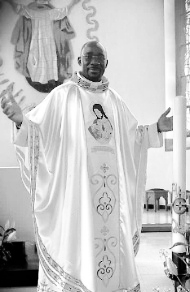
\includegraphics[scale=1.20]{../images/standing_daniel}
\end{wrapfigure}
Cette année nous porterons ensemble cette rentrée dans le cœur de chacun avec nos \textbf{jeunes pro}. Chacun à son rythme, selon ses possibilités et ses réalités mais avec un seul et même objectif : l’accomplissement de nos activités communautaires. Présentons également notre rentrée paroissiale au Christ. Et continuons notre chemin pour la mise en œuvre de notre projet paroissial autour de ce principal thème : \textbf{\og Avec notre jeunesse bâtissons une communauté plus dynamique, rayonnante et missionnaire\fg{}.}

	Que cette rentrée pastorale nous aide à prendre des résolutions nécessairement pour plonger à frais nouveaux dans la parole et être des disciples crédibles de l’évangile.


\begin{flushright}
Bonne rentrée pastorale à toutes et à tous !
\textit{Père  Daniel  ETTÉ}
\end{flushright}


\end{minipage}
%\end{center}
% -----
\end{document}
